% arara: pdflatex
% arara: convert: {density: 160, otheroptions: -dispose previous -delay 25 -loop 1, format: gif}
% arara: showfile: {format: gif}
\documentclass{article}
\usepackage[utf8]{inputenc} %probably not needed ...
\usepackage[T1]{fontenc}
\usepackage{geometry}
\geometry{papersize={128mm,96mm},margin=0.5cm} %\textwidth=11.8, \textheight=8.6
\usepackage{eso-pic}
\usepackage{tikzducks} 
\usetikzlibrary{arrows.meta,positioning, shapes.callouts, decorations.pathmorphing}
\usepackage{pgfplots}
\usetikzlibrary{pgfplots.fillbetween, intersections}

\newcommand{\devilduck}{%
\begin{scope}
\path (-2,0) -- ++(5,0) -- ++(0,5.5) -- ++(-5,0) -- cycle;
\duck[body=red, grumpy, bill=black, name=devil]
\filldraw[black] ([xshift=2pt]devil-head) to[bend right] +(6pt,6pt) to[bend left] +(-4pt,-8pt) to[bend left] cycle; 
\filldraw[black] ([xshift=-2pt, yshift=1pt]devil-head) to[bend left] +(-6pt,6pt) to[bend right] +(4pt,-8pt) to[bend right] cycle; 
\end{scope}%
}
\newcommand{\normalduck}{%
\begin{scope}[xshift=-11em]
\path (-1,0) -- ++(4.2,0) -- ++(0,5.5) -- ++(-4.2,0) -- cycle;
\duck[name=duck]	
\end{scope}%
}
\newcommand{\fork}[1]{%
\coordinate (forkpos) at ([xshift={#1}]devil-wing);
\draw[-Stealth, line width=1.6pt] (forkpos) -- ++(-2.5,0);
\draw[Stealth-Stealth, line width=1.6pt] ([shift={(-2.3,.3)}]forkpos) -- ++(.6,0) to[bend left]  ++(0,-.6) -- ++(-.6,0);%
}

\begin{document}
\AddToShipoutPictureBG{%
\AtPageLowerLeft{%
	
\begin{tikzpicture}[overlay,remember picture]
		\draw[red, very thick, name path=myborder] (0,0) rectangle (\paperwidth,\paperheight);
		\path[decorate, name path=myzigzag,
			decoration={zigzag,
				amplitude=.7cm,
				segment length=1.7cm
				}
			] 
			(1,1) rectangle (.92\paperwidth,.9\paperheight);
		\tikzfillbetween[of=myborder and myzigzag] {red};
		\end{tikzpicture}}}
\centering
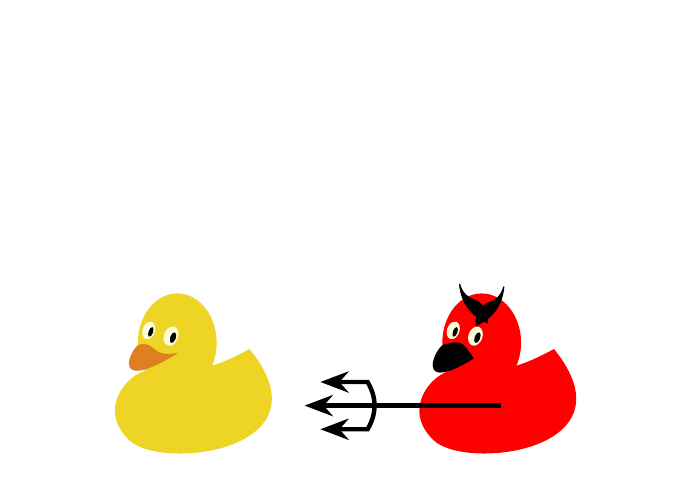
\begin{tikzpicture}	
	\devilduck
	\normalduck
	\fork{1em}
\end{tikzpicture}	
\newpage
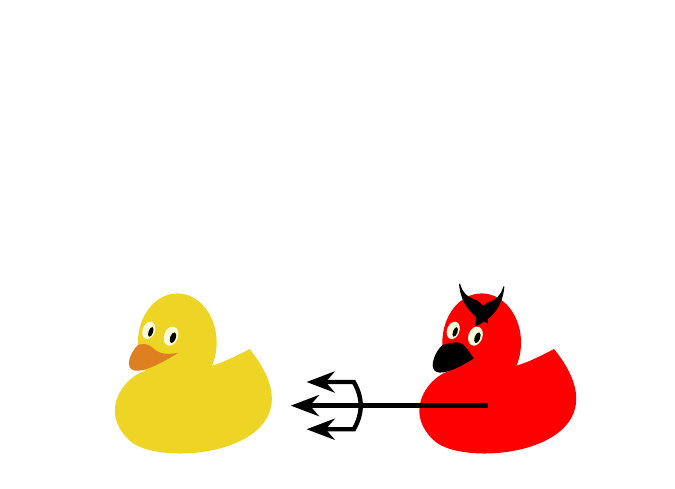
\begin{tikzpicture}	
	\devilduck
	\normalduck
	\fork{.5em}
\end{tikzpicture}	
\newpage
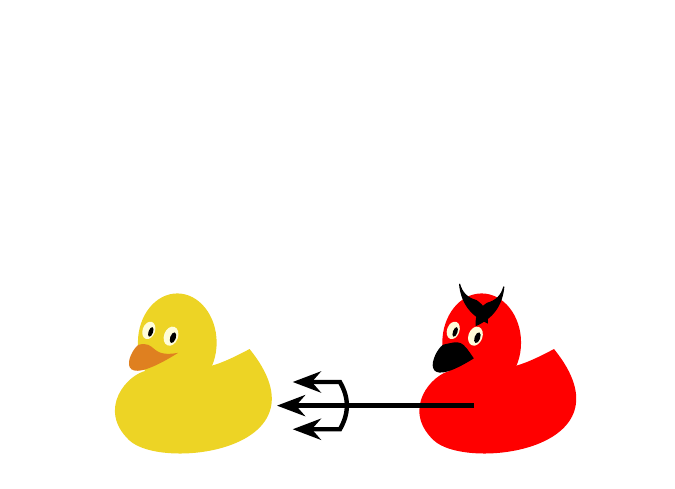
\begin{tikzpicture}[remember picture]
	\devilduck
	\normalduck
	\fork{0em}
\end{tikzpicture}
\begin{tikzpicture}[remember picture, overlay]
\node[ellipse callout, draw=blue, text=red] at ([shift={(-1,1)}]duck-head) {\textbf{Ouch!}};
\end{tikzpicture}
\end{document}
